\documentclass{article}
\usepackage[utf8]{inputenc}
\usepackage{geometry}
\geometry{
	a4paper,
	total={170mm,257mm},
	left=20mm,
	top=20mm,
}
\usepackage{graphicx}
\graphicspath{{images/}}
\usepackage{svg}
\usepackage{titling}
\usepackage[american,RPvoltages]{circuiTikz}
\usepackage{tikz, tikz-cd}
\usepackage{pgfplots}
\usepackage{siunitx}
\usepackage{float}
\usepackage{enumitem}
\usepackage{amsmath,amsfonts,stmaryrd,amssymb} % Math packages
\usepackage{tcolorbox}
\usepackage{pdfpages}
\title{Comparador de ventana}
\author{Rodrigo}
\date{Enero 2025}


\usepackage{fancyhdr}
\fancypagestyle{plain}{%  the preset of fancyhdr 
	\fancyhf{} % clear all header and footer fields
	\fancyfoot[L]{\thedate}
	\fancyhead[L]{Comparador de ventana}
	\fancyhead[R]{\theauthor}
}
\makeatletter
\def\@maketitle{%
	\newpage
	\null
	\vskip 1em%
	\begin{center}%
		\let \footnote \thanks
		{\LARGE \@title \par}%
		\vskip 1em%
		%{\large \@date}%
	\end{center}%
	\par
	\vskip 1em}
\makeatother


%\usepackage[color=red!20]{draftwatermark}
%\SetWatermarkText{CONFIDENTIAL\\COPY}
%\SetWatermarkScale{3}

\usepackage{lipsum}  
%\usepackage{cmbright}
%\usepackage{mathpazo}
%\usepackage{ccfonts,eulervm}
 \usepackage[T1]{fontenc}
 \usepackage{ccfonts}
%\usepackage[math]{anttor}
%\usepackage{antpolt}
 %\usepackage{fouriernc}
%\usepackage[utopia]{mathdesign}
%---------------------------------------------------
\tikzset{flipflop myRS/.style={flipflop,
		 flipflop def={t1=R, t3=S, t6=Q, t4={\ctikztextnot{Q}}, tu={\ctikztextnot{RST}}, nu=1, n4=1 }}
	}
	
\tikzset{flipflop myFFRS/.style={flipflop,
		flipflop def={t1=R, t3=S, t6=Q, t4={\ctikztextnot{Q}}, n4=1 }}
}
%---------------------------------------------------
\setlength\parindent{0pt}


\begin{document}
	
\maketitle
	
\noindent\begin{tabular}{@{}ll}
Author & \theauthor\\
\end{tabular}
	
\section*{Introducción}
Un comparador de ventana, también llamado \textit{detector de ventana} consiste usualmente de un par de comparadores de voltaje en paralelo (en configuración inversora y no inversora) para determinar si una señal se encuentra entre dos voltajes de referencia. Los niveles de voltaje entre estos dos voltajes de referencia superior e inferior es denominado como \textit{ventana}. Si la señal está dentro de la ventana, la salida es \texttt{ALTA}. Si la señal se encuentra fuera de la ventana, entonces la salida es \texttt{BAJA}.\\ 		 

Considere el circuito presentado en la figura 1. Para este diseño, los voltajes de referencia $V_{high}$ y $V_{low}$ son generados a partir de una fuente de alimentación simple combinada con divisores de voltaje. Es importante tener en cuenta que los comparadores deben ser de colector o drenador abierto para permitir la lógica cableada \texttt{AND}. 
\begin{figure}[H]
	\centering	
	\begin{tikzpicture}[scale=0.8]
		\ctikzset{bipoles/thickness=4}
		\ctikzset{monopoles/vcc/arrow={Stealth[width=6pt,length=9pt]}}
		\ctikzset{monopoles/vee/arrow={Stealth[width=6pt,length=9pt]}}
		\draw (0,0) node[op amp, noinv input up, anchor=out](OA1){$$};
		\draw[-latex] (OA1.up) -- +(0,1) node[above] (vv) {$V_{cc}$};
		\draw (OA1.down) -- +(0,-0.2) node[ground]{};
		\draw (OA1.-) to [short] ++(-1,0) coordinate (p1) to[short] ++(0,-4) coordinate (p2) to[short] ++(1,0) node[op amp, noinv input up, anchor=+](OA2){};
		\coordinate (M) at ($(p1)!0.5!(p2)$);
		\draw (M) to[short, *-] ++(-2,0) to[V, invert, l=$V_{IN}$] ++(0,-2) node[ground]{};
		\draw (OA1.out) to[short] (OA1.out |- OA2.out);
		\draw (OA1.+) to[short] ++(-5,0) coordinate (p3);
		\draw (OA2.-) to[short] ++(-5,0) coordinate (p4);
		\draw (p3) node[above right]{$V_{H}$} to[R, l_=$R_2$] (p4);
		\draw (p4) node[above right]{$V_{{L}}$} to[R, *-, l_=$R_1$] ++(0,-3) node[ground]{};
		\draw[-latex] (p3) to[R, *-, l=$R_3$] ++(0,3) node[above] (vv) {$V_{cc}$};
		\coordinate (M1) at ($(OA1.out)!0.5!(OA2.out)$);
		\draw (M1) to[short, *-o] ++(3,0) coordinate (p4) node[right]{$V_o$};
		\coordinate (M2) at ($(M1)!0.5!(p4)$);
		\draw[-latex] (M2) to[R, l_=$R_p$, *-] ++(0,4) node[above] (vv) {$V_{pu}$};
		\draw[-latex] (OA2.up) -- +(0,1) node[above] (vv) {$V_{cc}$};
		\draw (OA2.down) -- +(0,-0.2) node[ground]{};
	\end{tikzpicture}
	\caption{Comparador de ventana básico}	
	\label{fig:figura1}
\end{figure}

El voltaje de ventana inferior está dado por

\begin{align}
	V_L = \frac{R_1 V_{cc}}{R_1 + R_2 + R_3}
\end{align}

El voltaje de ventana superior está dado por
\begin{align}
	V_H = \frac{(R_1 + R_2) V_{cc}}{R_1 + R_2 + R_3}
\end{align}

Cuando el voltaje de entrada se encuentre entre $V_H$ y $V_L$ la salida será \texttt{ALTA}. Cuando el voltaje de entrada esté fuera de dicho rango, la salida será puesta a tierra.


Si resolvemos las ecuaciones (1) y (2) para $V_{cc}$ obtenemos

\begin{align}
	V_{cc} = \frac{(R_1 +R_2 + R_3)V_L}{R_1} \\
	V_{cc} = \frac{(R_1 +R_2 + R_3)V_H}{R_1 + R_2} 
\end{align}

Al igualar ambas ecuaciones obtenemos

\begin{align}
	\frac{(R_1 +R_2 + R_3)V_L}{R_1} &= \frac{(R_1 +R_2 + R_3)V_H}{R_1 + R_2}  \\
	\frac{V_L}{R_1} &= \frac{V_H}{R_1 + R_2}
\end{align}

Así, la relación entre $V_H$ y $V_L$ es

\begin{align}
	\frac{V_H}{V_L} = \frac{R_1 + R_2}{R_1} = 1 + \frac{R_2}{R_1}
\end{align}

Para calcular el valor de $R_3$, podemos despejar $R_3$ de la ecuación (1) o (3), por ejemplo

\begin{align}
	V_{cc} &= \frac{(R_1 +R_2 + R_3)V_L}{R_1} \nonumber \\
	\frac{V_{cc}}{V_L} &= \frac{R_1 +R_2 + R_3}{R_1} \nonumber \\
	\frac{R_1V_{cc}}{V_L} &= R_1 + R_2 + R_3 \nonumber
\end{align}

O bien

\begin{align}
	R_3 = \frac{R_1V_{cc}}{V_L} - (R_1 + R_2)
\end{align}

\section*{Ejemplo 1}
Diseñe un comparador de ventana de manera que detecte una señal de voltaje en el rango de $V_L=\qty{5}{\volt}$ y $V_H=\qty{7}{\volt}$ \\

La relación entre $V_H$ y $V_L$ es
\begin{align}
	\frac{V_H}{V_L} = \frac{\qty{7}{\volt}}{\qty{5}{\volt}} = 1 + \frac{R_2}{R_1} = 1.4 \nonumber
\end{align}

Y la relación entre los resistores $R_2$ y $R_1$ es

\begin{align}
	\frac{R_2}{R_1} = 1.4 - 1 &= 0.4 \nonumber \nonumber \\
	R_2 &= 0.4R_1
\end{align}

Haciendo $R_1$ = \qty{10}{\kilo \ohm}, entonces $R_2 = \qty{4}{\kilo \ohm}$. Por último, calculamos el valor de $R_3$

\begin{align}
	R_3 = \frac{(\qty{10}{\kilo \ohm})(\qty{12}{\volt})}{\qty{5}{\volt}} - (\qty{10}{\kilo \ohm} + \qty{4}{\kilo \ohm}) = \qty{10}{\kilo \ohm}
\end{align}

\begin{figure}[H]
	\centering
	% trim=left botm right top
	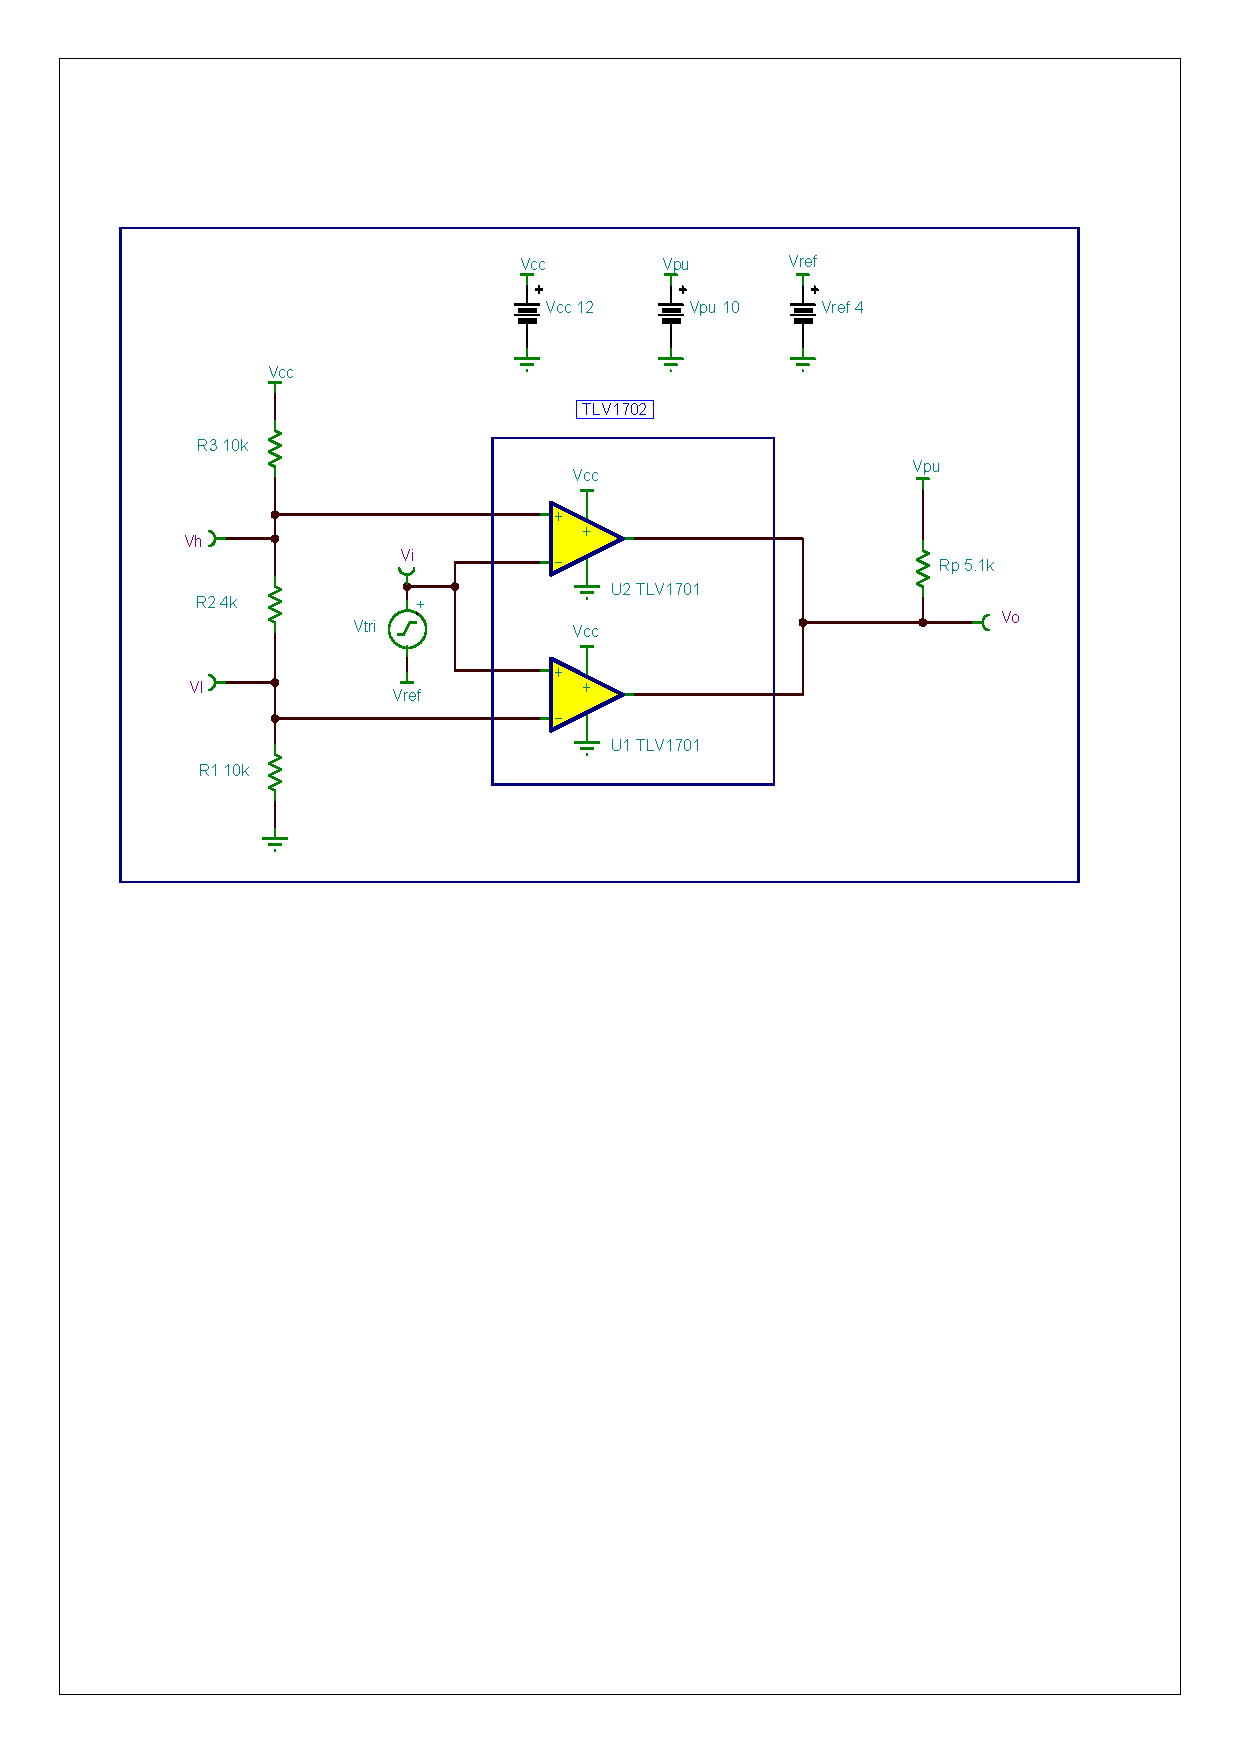
\includegraphics[clip, trim=3cm 15cm 3.5cm 4cm, width=\textwidth]{TINA Diagram2}
	\caption{Diagrama esquemático}	
	\label{fig:figura2}
\end{figure}

\begin{figure}[H]
	\centering
	% trim=left botm right top
	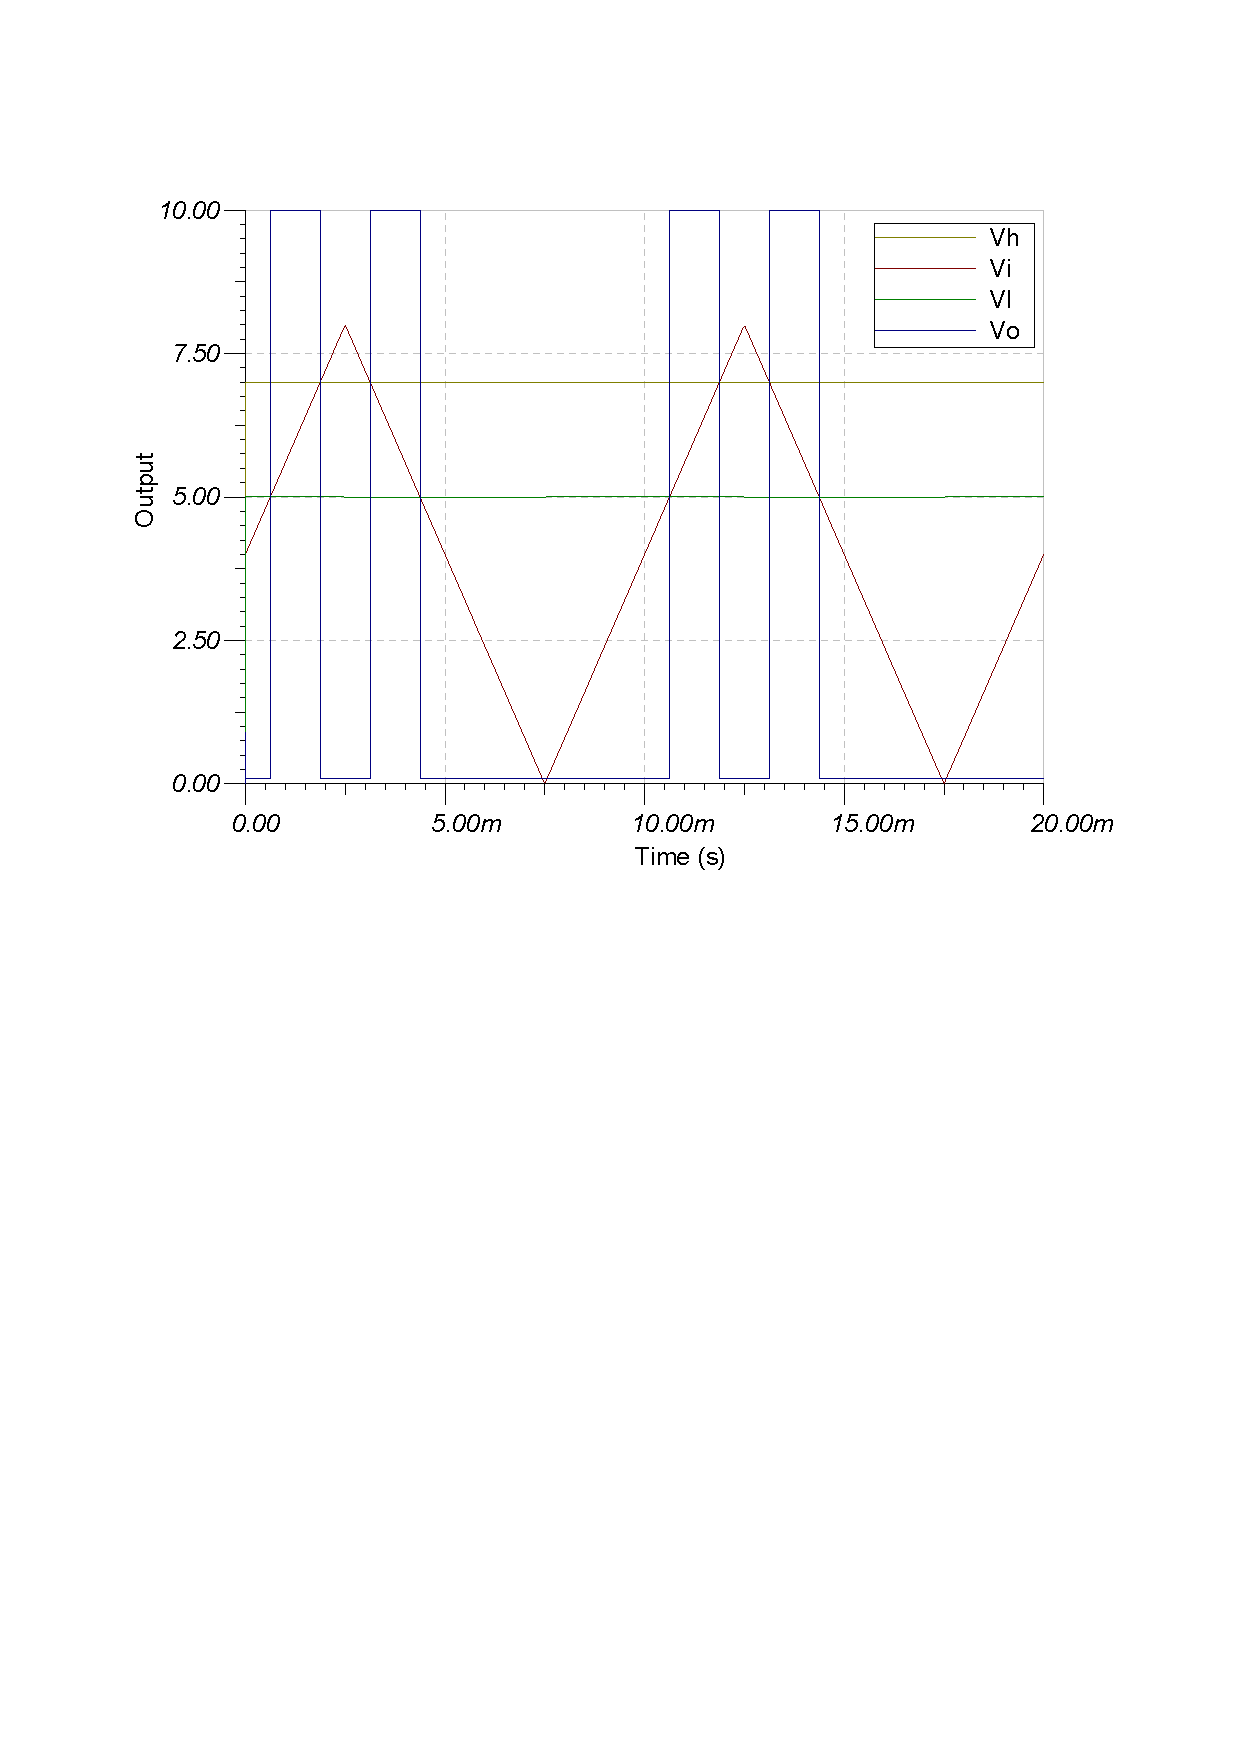
\includegraphics[clip, trim=1.5cm 15cm 2cm 3cm, scale=0.9]{TINA Diagram1}
		\caption{Formas de onda}	
	\label{fig:figura3}
\end{figure}

\end{document}